\documentclass[hidelinks,12pt]{article}
\usepackage{amsmath}
\usepackage{graphicx}
\usepackage[english]{babel}
\usepackage[utf8]{inputenc}
\usepackage{fancyhdr}
\usepackage{tabularx}
\usepackage{hyperref}
\usepackage{float}
\usepackage{subcaption}
\usepackage{listings}
\usepackage{xcolor}

\definecolor{codegreen}{rgb}{0,0.6,0}
\definecolor{codegray}{rgb}{0.5,0.5,0.5}
\definecolor{codepurple}{rgb}{0.58,0,0.82}
\definecolor{backcolour}{rgb}{0.95,0.95,0.92}

\lstdefinestyle{mystyle}{
    backgroundcolor=\color{backcolour},   
    commentstyle=\color{codegreen},
    keywordstyle=\color{magenta},
    numberstyle=\tiny\color{codegray},
    stringstyle=\color{codepurple},
    basicstyle=\ttfamily\footnotesize,
    breakatwhitespace=false,         
    breaklines=true,                 
    captionpos=b,                    
    keepspaces=true,                 
    numbers=left,                    
    numbersep=5pt,                  
    showspaces=false,                
    showstringspaces=false,
    showtabs=false,                  
    tabsize=2
}

\lstset{style=mystyle}

\hypersetup{
    colorlinks=true,
    linkcolor=cyan,
}

\pagestyle{fancy}
\fancyhf{}
\chead{DRAM Request Manager for Multicore Processors}
\rfoot{\thepage}

\begin{document}

\begin{titlepage}
    \centering
    
\includegraphics[scale=0.5]{../../logo.png}\\[1.0cm]
    \Large INDIAN INSTITUTE OF TECHNOLOGY DELHI\\[1.0 cm]
    \LARGE COL216\\[0.1cm]
    \Large \underline{Report}\\
    \large \[Assignment-5\]
    \LARGE \textbf{DRAM Request Manager for Multicore Processors}


    \rule{\textwidth}{0.2 mm} \\[0.1cm]
    \begin{abstract}
        A simulator is a software that emulates the actions of an entity without actually utilising the entity.
        Here we attempt to create a cross platform MIPS simulator that emulates all the hardware instructions supported by MIPS.
        This simulator takes as input a MIPS assembly program that translates it into instructions executed by MIPS.
        \\[0.1cm]
    \end{abstract}
    \rule{\textwidth}{0.2 mm} \\[0.1cm]
    \begin{flushright}

        \begin{tabular}{c|c}
            \small {Harsh Agrawal}      & \small {2019CS10431} \\
            \small {Saptarshi Dasgupta} & \small {2019CS50447} \\
        \end{tabular}
    \end{flushright}
\end{titlepage}
\tableofcontents
\newpage
\section{Overview}
This assignment extends the earlier DRAM Driver to the multicore CPU
case. The architecture now consists of $N$ CPU cores, each running a different MIPS program,
and sending DRAM requests to a DRAM Driver which interfaces with the DRAM

\section{Modules}
We implemented a simulator in \verb|C++| for executing MIPS instructions from assembly code. The program was divided into \verb|compiler| ,\verb|hardware|, \verb|DRAM| and a \verb|DramDriver| module.
These modules perform different functions as outlined below
\subsection{Compiler}
\begin{itemize}
    \item This module takes as input the assembly program and parses the tokens according to the syntax specifications of MIPS assembly programs.
    \item This module assembles the program into a sequence of instructions that can be executed according to the hardware specifications.
    \item It also generates appropriate syntax errors if an erreneous expression or an unidentified token is encountered.
    \item The compiler checks the encodibility of instructions into 4 bytes (without actually encoding it) using the size of operands involved.
\end{itemize}
\subsection{Hardware}
\begin{itemize}
    \item This module emulates a subset of instructions provided by MIPS. They are \verb|add, mul, sub, slt, addi, bne, beq, j, lw, sw|.
    \item The module maintains a record of all the register and memory values and modifies them according to the instruction specifications.
    \item It generates appropriate exceptions on performing prohibited actions like out of bounds memory access and reserved register access.
\end{itemize}

\subsection{DRAM}
\begin{itemize}
    \item This module implements the DRAM model in the form of a \verb|2D| array.
    \item It contains a row buffer to simulate an actual \verb|DRAM|. A row is first copied into this row buffer and the module uses the buffer as a write-back cache for further read and write operations.
\end{itemize}

\subsection{DramDriver}
\begin{itemize}
    \item A \verb|DramDriver| module is implemented to capture all \verb|DRAM| requests from all cores and reorder them according to some pre determined heuristics.
    \item It is equipped with all optimizations to give the best performance. It includes forwarding, eliminating redundant \verb|LW| and \verb|SW| instructions.
    \item It also protects against starvation by appropriately context switching out DRAM requests of a core.
    \item It automaticaly converts the virtual address space to the physical address space before queuing in a memory request.
\end{itemize}

\section{Approach}

The approach used to implement the \verb|DramDriver| for multicore processors is described in this section.
\subsection{Data}
We propose to implement the \verb|DramDriver| in hardware using a few lookup tables and some queues for storing the pending requests.
The data modules required by our implementation are described in detail below.
\subsubsection{Queues}
$8$ queues, each with a size of $8$ requests. This gives us a space for exactly $64$ requests at a time.
Queues need to be of finite size since we would have hardware supporting only a finite size and any implementation with an infinite size assumption is infeasible to implement.

We have supported random access to queued requests and a request can be enqueued at any index. This just invoves changing the stored register value from a register file.
Each queue can be indexed using a multiplexor as done in a cache.
We have also assumed random access of any of the 8 elements of the queue which is easy to implement.
A queue holds all the requests of the same row. Hence every queue deals with a different row of the DRAM and this makes it easier to schedule requests.

The decision for the size of each queue and the number of queues was taken keeping in mind the hardware constraints and design principle \textit{Smaller is faster}
However, our implementation is completely modular, and by changing just one value we can simulate the Driver with some other values to
test which one seems to give the best throughput.

\subsubsection{Look-up Tables}

The state of the queues is maintained using several lookup tables which can be easily implemented in the hardware using multiplexors and is also used in many practical hardware implementations.
The description of each look up table along with its corresponding name in our simulator code is given below.
Assume $N$ is the number of cores in the processor.
\begin{table}[H]
    \begin{tabular}[]{|c|c|p{0.2\linewidth}|p{0.4\linewidth}|}
        \hline
        LUT name                & Size          & Index                    & Stored value                                                                                                                   \\  \hline \hline
        \verb|__core2freq_LUT| & $N $          & core number              & Frequency of DRAM accesses (\verb|lw|/ \verb|sw|)                                                  \\ \hline
        \verb|__core2instr_LUT| & $N $          & core number              & Number of instructions executed.                                                                                               \\ \hline
        \verb|__core2PA_offsets_LUT| & $N $          & core number              & Virtual to physical address offset.                                                                                            \\ \hline
        \verb|__core2blocked_reg_LUT| & $N \times 3$  & core number              & The set of blocked registers.                                                                                                  \\ \hline
        \verb|__queue2row_LUT| & $8 $          & queue number             & row of requests in the queue.                                                                                                  \\ \hline
        \verb|__queue2size_LUT| & $8 $          & queue number             & Number of active requests in the queue                                                                                         \\ \hline
        \verb|__core_reg2offsets_LUT| & $N \times 32$ & (core num, register num) & Returns the (queue number, index in queue) pair of a \verb|lw| request involving the given register of the core. \\ \hline
    \end{tabular}
    \caption{Description of LUTs}
\end{table}

\subsection{Control}
This section specifies how the data modules are used to implement the queuing model for DRAM requests.
The following points briefly illustrate the working of our model. Assume that the relevant lookup tables are updated
at each operation, the exact details of which are skipped here for simplicity.
\begin{itemize}
    \item When a request is received, the row number is checked and a queue is searched with the given row, this can be done parallely in hardware using
          8 comparators attached to the \verb|__queue2row_LUT|. If a queue is found with the row, a push operation is attempted in the queue, if the queue is full then
          an exception is thrown which signals the processor that it should retry the request once the queue has some space.
    \item When a request is completed it is removed from the queue (pop), updating the relevant lookup up tables to ensure correctness.
    \item The queue switching logic takes into account the blocked registers of each core (\verb|__core2blocked_reg_LUT|), the number of instructions executed by a core (\verb|__core2instr_LUT|), the frequency of DRAM accesses by a core (\verb|__core2freq_LUT|)
          and creates a combined metric to decide the next queue. All this logic can be handled by a combinational circuit and is feasible to implement in hardware.
    \item The switching logic first tries to schedule the queue that has a blocking request. However, if multiple queues with such requests exist then the core with the lowest frequency of DRAM accesses and largest number of instructions is chosen (to increase the throughput).
          When scheduling a queue we try to execute the requests that are blocking a processor over other requests. However, if there is a dependency conflict then a compromise has to be made and other requests have to be executed.
    \item The circuits also incur a delay of some clock cycles and a busy bit is maintained inside the controller. When the controller is busy, it does not accept any more requests, and generates an exception.
\end{itemize}
\newpage
\subsection{Optimizations}

We have also implemented several optimizations to eliminate redundant work for increasing the throughput.

\begin{itemize}
    \item \verb|Forwarding:| Whenever we recieve a \verb|lw| for an address such that a \verb|sw| for it already exists in our queue, we do not enqueue the \verb|lw| request in the queue and instead forward the value directly to the corresponding register
          from the value stored in the \verb|sw| request in the queue.
    \item \verb|Redundant sw:| Before inserting a \verb|sw| request in the queue we lookup for a matching \verb|sw| request in the queue and nullify the searched request.
    \item \verb|Redundant lw:| Before inserting a \verb|lw| request in a queue, a matching \verb|lw| request is obtained using the \verb|__core_reg2offsets_LUT| lookup table.
          If the lookup table contains valid entries the request corresponding to the matching request is nullified.
    \item \verb|Starvation:| The driver executes all requests in the current queue. However to prevent starvation a counter is maintained each time a request is completed,
          if this counter exceeds the queue size then the queue is switched out and some other queue is chosen to execute requests.
\end{itemize}

\textbf{Note:} Since the queue size is finite ($8$) looking up a request in a queue can be implemented using $8$ comparators which would operate parallely to check for the required conditions.

\subsection{Hardware implementation model}
This section illustrates the circuit models that can be used to implement the driver on real hardware.

We have shown several modules as black boxes but we believe most of them can be implemented using simple combinational circuits,
and the exact details have been skipped for clarity.
\begin{figure}[H]
    \centering
    \begin{subfigure}[h]{\textwidth}
        \begin{center}
            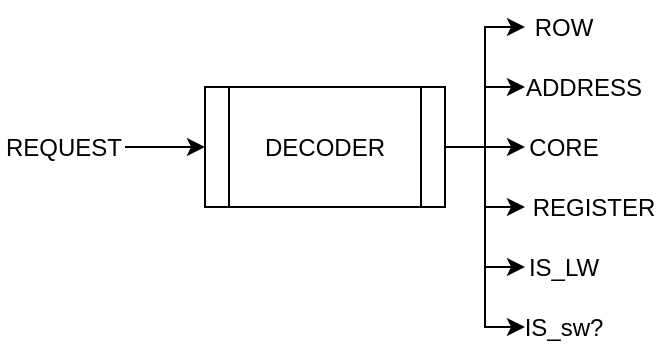
\includegraphics[scale=0.4]{img/decoder.png}
            \caption{\textbf{Decoder}: Recieves the encoded request and extracts the parameters that can be used by other modules}

        \end{center}

    \end{subfigure}

    \begin{subfigure}[h]{\textwidth}
        \begin{center}
            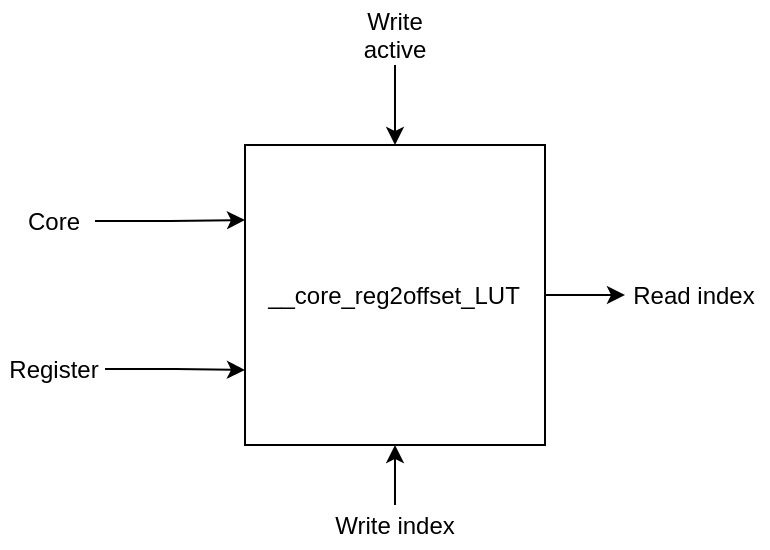
\includegraphics[scale=0.4]{img/core_reg_LUT.png}
            \caption{\textbf{LW index store LUT}: Stores the queue numbers and queue indices of LW requests. It can be indexed by core and register number. }

        \end{center}

    \end{subfigure}

\end{figure}
\begin{figure}[H]
    \ContinuedFloat
    \centering

    \begin{subfigure}[h]{\textwidth}
        \begin{center}
            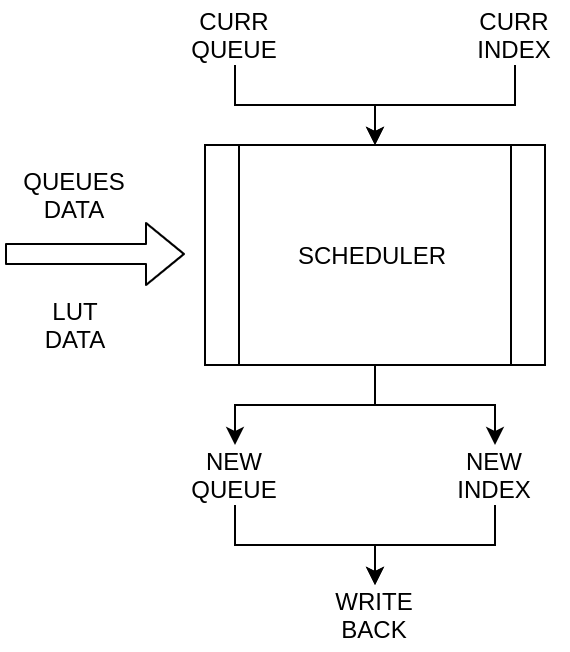
\includegraphics[scale=0.4]{img/scheduler.png}
            \caption{\textbf{Scheduler}: Takes as input the current queue and index and schedules the next queue and index based on some LUTs and the requests in queue.}

        \end{center}

    \end{subfigure}
    \begin{subfigure}[h]{\textwidth}
        \begin{center}
            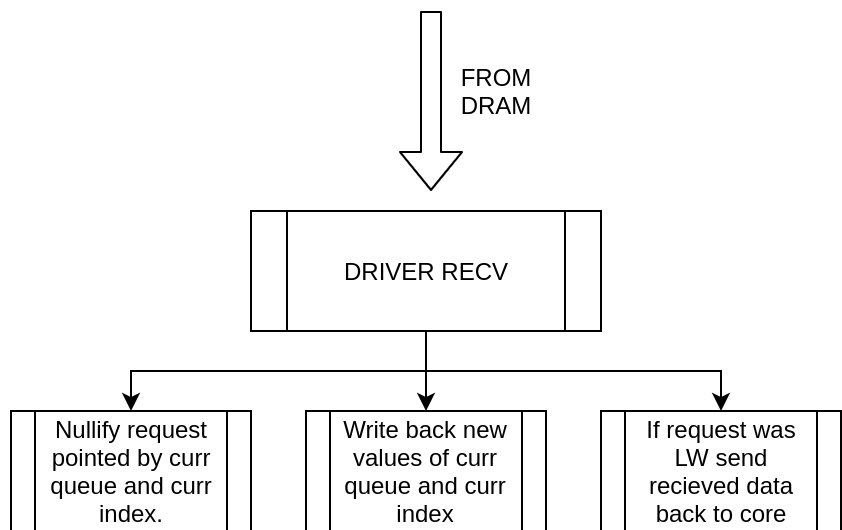
\includegraphics[scale=0.3, trim = 0 0 10 0]{img/dram_recv.png}
            \caption{\textbf{Dram recieve}: Recieves data from DRAM and takes appropriate action}

        \end{center}

    \end{subfigure}

\end{figure}

\begin{figure}[H]
    \ContinuedFloat
    \centering

    \begin{subfigure}[h]{\textwidth}
        \begin{center}
            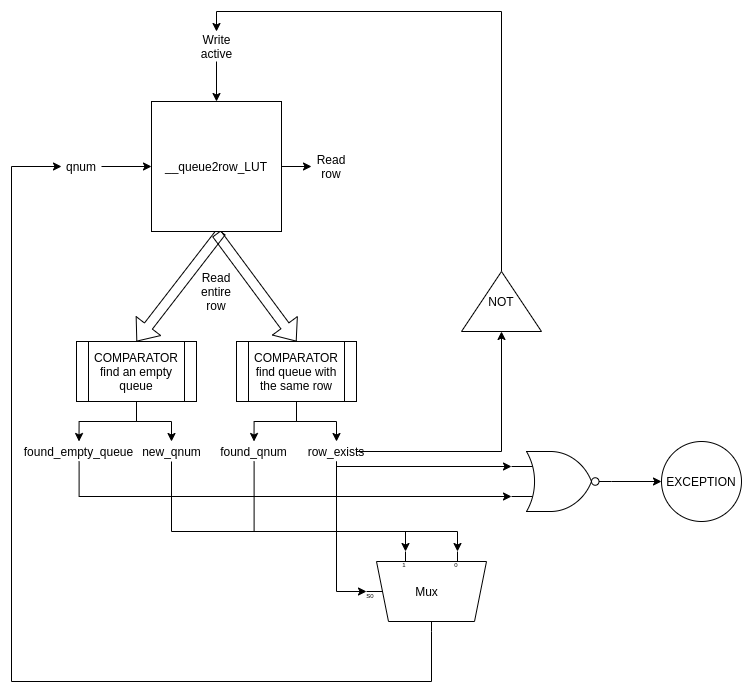
\includegraphics[scale=0.65]{img/queue_selector.png}
            \caption{\textbf{Queue selector}: Selects the queue to insert the incoming request into. Raises exception if no queue is empty.}

        \end{center}

    \end{subfigure}
\end{figure}

\begin{figure}[H]
    \ContinuedFloat
    \centering

    \begin{subfigure}[h]{\textwidth}
        \begin{center}
            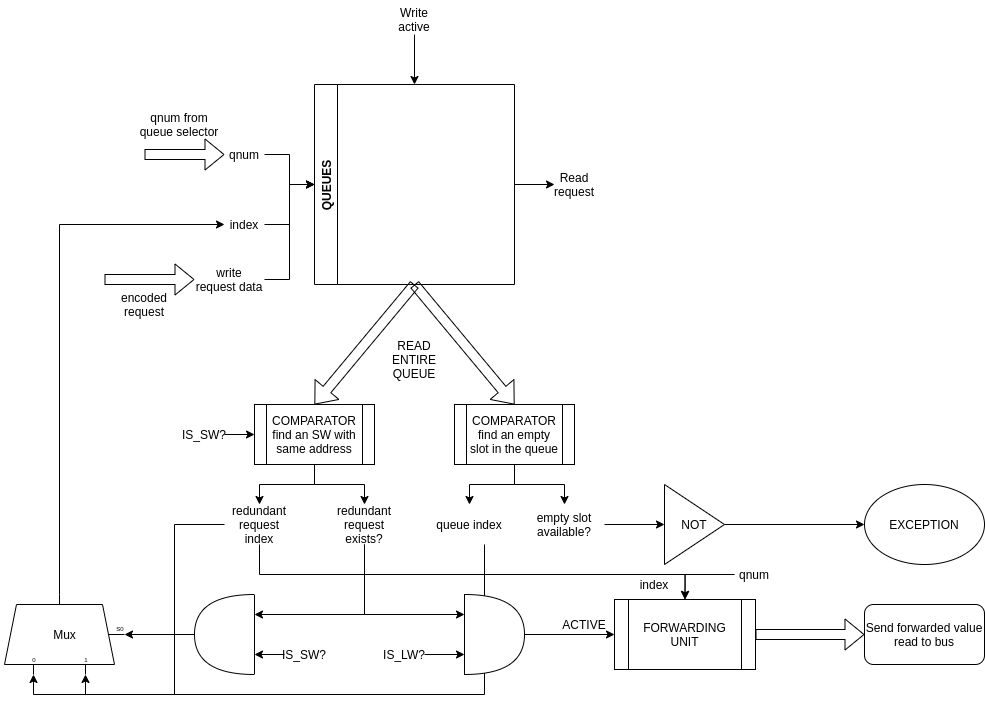
\includegraphics[scale=0.5]{img/enqueue.png}
            \caption{\textbf{Enqueue}: Enqueue the request into the appropriate queue. Implements forwarding and elimination of redundant SW requests.}

        \end{center}

    \end{subfigure}
    \begin{subfigure}[h]{\textwidth}
        \begin{center}
            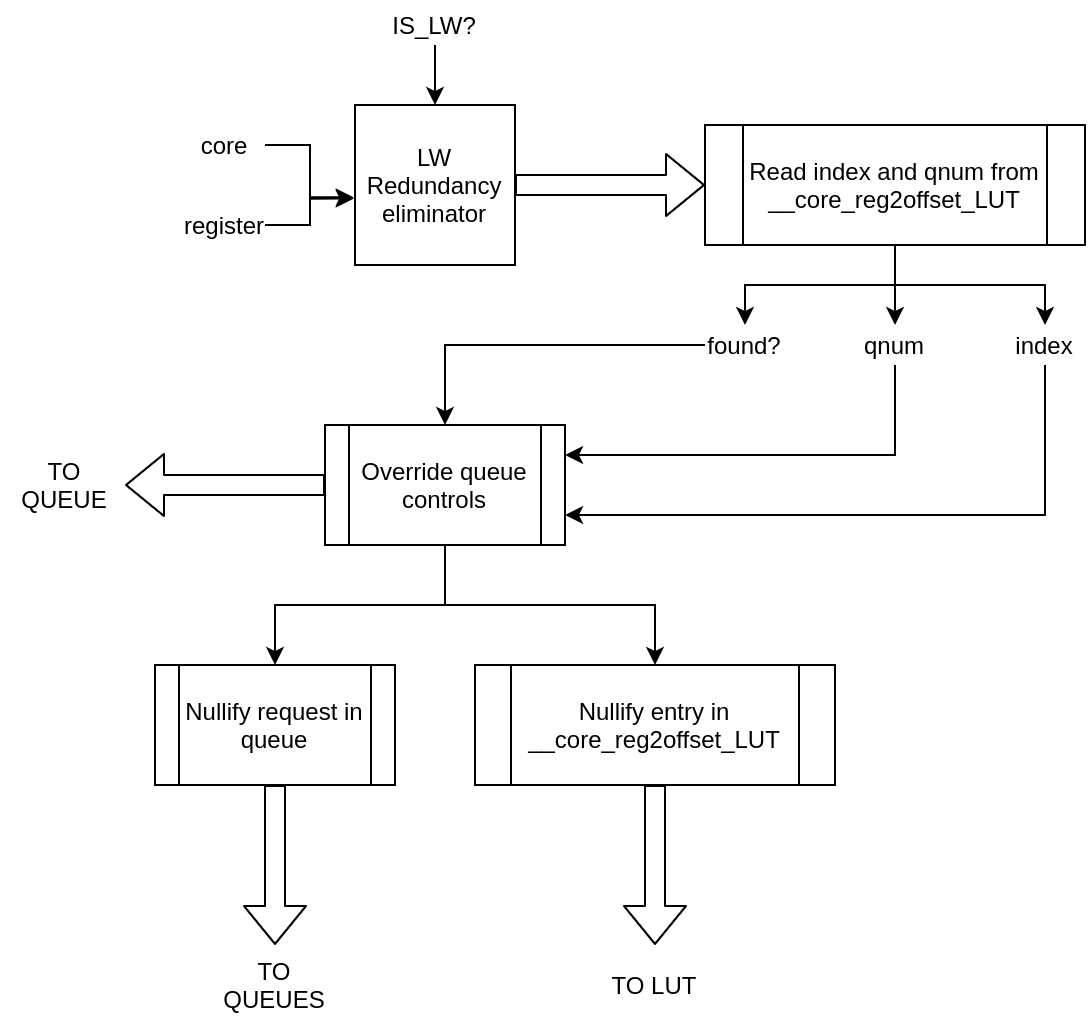
\includegraphics[scale=0.23]{img/lw_redundancy.png}
            \caption{\textbf{Redundant LW}: eliminates redundant LW instructions.}

        \end{center}

    \end{subfigure}
\end{figure}
\subsection{Delay estimation}
In this section we try to estimate the delay incurred by each stage of the DRAM driver. We have attempted to decrease the delay times as far as possible.
However, due to these delays, the DRAM driver will remain busy for some clock cycles and until then it won't be able to accept any requests.

\begin{enumerate}
    \item \textbf{Queue selection:} The circuit selects a queue from the available queues to enqueue the incoming request.
          This process just requires reading the \verb|__queue2row_LUT| and writing to it at the end of the clock cycle if a new row has to be allocated. The estimated delay is \textbf{1 clock cycle}.
    \item \textbf{Enqueue:} The enqueue operation determines the appropirate index in the queue by reading the entire queue and passing it through comparator circuits.
          It searches for a redundant SW request, and if found then forwards the values to the register file. If a redundant SW request is found, its contents are replaced by the incoming request.
          Once the index is determined, the request is written to the queue block at the end of the clock cycle. The estimated delay is \textbf{1 clock cycle} each.
          However, if a redundant LW request is eliminated, the existing request needs to be nullified before the new request can be written to the queue.
          This constitutes two writes to the same data structure and hence incurs a delay of \textbf{2 clock cycles}.
    \item \textbf{Request completion:} The driver recieves data from the DRAM and completes the request. It involves writing to the queues, updating several registers and LUTs.
          The controller can set the control signals appropriately and all data would be updated in \textbf{1 clock cycle}.
    \item \textbf{Scheduler:} The scheduler reads the values of current queue and index and resets them to prevent \textit{starvation}.
          It also analyses the data from each queue and combines them with data stored in the LUTs, to produce a priority measure. This is done by a logical arithmetic circuit which requires several floating point operations and hence cannot be completed in a single clock cycle.
          The delay will depend on the implementation of floating point operations and hence is dependent on the hardware implementation of arithmetic operations.
          A rough estimate is 2 clock cycles and along with one clock cycle for writing to the registers, the estimated delay is \textbf{3 clock cycles}.
\end{enumerate}

\subsection{Advantages}
\begin{itemize}
    \item The approach ensures that the overall throughput is maximized.
    \item The optimizations to replace requests pertaining to the same addresses or registers eliminate redundant requests thus further reducing the runtime without affecting the correctness.
    \item Forwarding enables us to entirely skip going to the DRAM and fetching the value directly in a short period of time.
    \item Eliminating starvation ensures that a single core does not eat up all the resources on a DRAM driver.
    \item The sophisticated scheduling logic incorporates all parameters (instruction access count, frequency of DRAM accesses, presence of blocking requests) and combines them to generate a measure that is compared to decide the next queue in schedule. This metric plays an essential role in determining the throughput.
    \item We always try to unblock a core first and in order to do that we start executing from the blocked requests in a queue while scheduling rows. This allows a processor to unblock as fast as possible and give the maximum throughput possible.
\end{itemize}
\subsection{Disadvantages}
\begin{itemize}
    \item Our approach will be useful for programs with large number of instructions and comparing the throughput on small programs could give incorrect interpretations.
    \item We would need a relatively complex hardware comprising 6 Lookup tables 8 queues and several comparators, which might increase the duration of a single clock cycle.
    \item Our approach does not optimally select the request that gets accepted into the Dram Driver if multiple cores issue a request in the same cycle.
\end{itemize}
\section{Testing}

The testing method was completely manual. The test cases written manually are included in the \verb|./tests/input| directory. The test cases were run with different parameters
of the program and the outcomes were compared.
\begin{itemize}
    \item \verb|deletion_lw:| this contains 3 test files to check for the optimization of deleting redundant LW instructions to the same register (by the same CORE) .
    \item \verb|deletion_sw:| this contains 3 test files to check for the optimization of deleting redundant SW instructions to the same memory address (by the same CORE).
    \item \verb|forwarding:| this contains 3 test files to check for forwarding LW instructions from previous SW instruction to the same address is present in the Dram Driver.
    \item \verb|manycores:| this contains 8 test files to demonstrate how our Dram Driver handles requests from large number of cores.
    \item \verb|optimal_switch_blocking:| this contains 2 test files to show how our Dram Driver switches queues when some queues contain blocking registers.
    \item \verb|optimal_switch_non_blocking:| this contains 2 test files to show how our Dram Driver switches queues when no queue contains blocking registers.
    \item \verb|single_write_port:| this demonstrates that only one of DRAM, Dram Driver and Processor can write to the register file at a particular clock cycle.
    \item \verb|starvation:| this demonstrates how our Dram Driver behaves when only requests from a single core are being processed for some time  .
    \item \verb|switch_with_loops:| this demonstrates a scenario with multiple LW and SW instructions inside loops.
\end{itemize}

\subsection{Result}
The program output was observed and all the register, memory and row buffer values were inspected for correctness manually. In each of the test case the expected outputs matched.\\[0.2cm]
The output logs of the test cases are available in the \verb|./tests/output| directory. The test cases were run with different configuration options.

\section{Assumptions}
\begin{itemize}
    \item We have assumed private physical spaces for each core, and this is achieved by dividing the total available memory into equal parts between each core. Although, in real implementations this would be done using a page table and the memory allocation is handled by the OS, but for simulation purposes our assumption is quite reasonable and shouldn't affect simlulation of ordinary programs.
    \item We have assumed that the maximum memory available to any user program is $2^{20}$ bytes. This does not include the memory required for storing instructions.
    \item We have assumed 32 registers for MIPS each of them storing 32 bits. We have hardwired the register \verb|$zero| to the value $0$ as is the case in MIPS hardware. We have also restricted use of kernel reserved registers \verb|$26, $27|.
    \item We have assumed that exactly 1 clock cycle is required for each of the instructions except \verb|lw, sw| to display the execution statistics.
    \item We have enforced tight syntax rules to enforce good coding practice. We disallow certain instructions like (a) \verb|lw $t1, ($sp)| and (b) \verb|lw $t1, 40231|.
          The first instruction skips supplying the offset to the register and the second one involves raw memory access.
    \item We have enforced the use of a whitespace between the operand and its arguments. For example \verb|add$t1,$t2,$t3| is disallowed as there is no whitespace between \verb|add| and \verb|$t1|
    \item We have implemented branching instructions like \verb|beq, bne, j| to take only labels and instruction numbers as the last argument.
\end{itemize}

\end{document}

